%%==============================================================
%% Modelo de TCC para o curso de Sistemas de Informação
%% da Universidade Federal de Viçosa - Campus de Rio Paranaíba
%% Autor: Rodrigo Smarzaro (smarzaro@ufv.br)
%% Última versão Março/2014
%% Arquivo em formato UTF-8
%% Compilar com pdftex
% %Precisa do arquivo UFV.sty
%%==============================================================

\documentclass[
	% -- opções da classe memoir --
	12pt,				    % tamanho da fonte
	openright,			    % capítulos começam em pág ímpar (insere página vazia caso preciso)
	oneside,			    % para impressão só no anverso. Oposto a twoside
	a4paper,			    % tamanho do papel.
    % -- opções do pacote abntex2 --
    % chapter=TITLE,         % Títulos em maiúsculas
    sumario=tradicional,    % Sumário padrão memoir (mais bonito "imo")
    % -- opções do pacote babel --
	english,			    % idioma adicional para hifenização
	brazil,				    % o último idioma é o principal do documento
	]{abntex2}              % Personaliza a capa. Precisa do arquivo ufv.cls para funcionar.



% Pacotes fundamentais
\usepackage{abntex2-UFV}        % Personalização para a Universidade Federal de Viçosa
\usepackage{lmodern}			% Usa a fonte Latin Modern			
\usepackage[T1]{fontenc}		% Selecao de codigos de fonte de saída
\usepackage[utf8]{inputenc}		% Codificacao do documento (conversão automática dos acentos)
\usepackage{indentfirst}		% Indenta o primeiro parágrafo de cada seção.
\usepackage{graphicx}			% Inclusão de gráficos
\usepackage{booktabs}           % \toprule, \midrule e \bottomrule para tabelas
% Sistema autor-data com títulos nas referências em negrito
\usepackage[alf,abnt-emphasize=bf]{abntex2cite}	


% ---
% CONFIGURAÇÕES DE PACOTES
% ---

% Informações de dados para CAPA e FOLHA DE ROSTO
\titulo{SheSafe – Aplicativo de pedido de ajuda para mulheres em situação de risco}
\autor{Lucas de Oliveira Macêdo}
\local{São Carlos}
\data{2025}
\orientador{Silvana Maria Affonso de Lara}    % redefinido no abntex2-UFV para aceitar Instituição (default = UFV-CRP)
%\coorientador{Nome do Coorientador}
\instituicao{Instituto Federal de São Paulo}

\campus{\emph{Campus} de São Carlos}      % pacote abntex2-UFV
\curso{Pós-Graduação \emph{Lato Sensu} em
Desenvolvimento de Sistemas para Dispositivos Móveis}               % pacote abntex2-UFV
\membrobancaA{Membro da Banca A}             % pacote abntex2-UFV default = UFV-CRP
\membrobancaB[UFMG]{Membro da Banca B}       % pacote abntex2-UFV default = UFV-CRP
\databanca{\today}                           % pacote abntex2-UFV

% O preambulo deve conter o tipo do trabalho, o objetivo,
% o nome da instituição e a área de concentração
\preambulo{Trabalho de conclusão apresentado ao Instituto Federal de São Paulo para obtenção do título de Especialista em Desenvolvimento para Dispositivos Móveis. }
% ---

% ---
% Configurações de aparência do PDF final

% informações para o arquivo pdf de saída
% Interessante alterar a cor dos links para preto(black)
% para imprimir
\makeatletter
\hypersetup{
        % metadados
		pdftitle={\@title},
		pdfauthor={\@author},
    	pdfsubject={\imprimirpreambulo},
	    pdfcreator={LaTeX with abnTeX2},
		colorlinks=true,   % false: links em frame; true: links coloridos
    	linkcolor=black,    % cor dos links no documento
    	citecolor=blue,    % cor dos links para a bibliografia
    	filecolor=magenta, % cor dos links para arquivos
		urlcolor=blue,     % cor dos links para sites
		bookmarksdepth=4   % profundidade do sumário do PDF
}
\makeatother
% ---

\begin{document}
% Retira espaço extra obsoleto entre as frases.
\frenchspacing

% ----------------------------------------------------------
% ELEMENTOS PRÉ-TEXTUAIS
% ----------------------------------------------------------
\pretextual

% Capa
\imprimircapa

% Folha de rosto
\imprimirfolhaderosto
% ---

% Inserir folha de aprovação
%\imprimirfolhadeaprovacao

% Dedicatória
%\begin{dedicatoria}
%   \vspace*{\fill}
%   \centering
%   \noindent
%   \textit{Texto qualquer da dedicatória}
%   \vspace*{\fill}
%\end{dedicatoria}
% ---

% Agradecimentos
%\begin{agradecimentos}

%\end{agradecimentos}
 ---

% Epígrafe
%\begin{epigrafe}
%    \vspace*{\fill}
%	\begin{flushright}
%		\textit{``Word? nunca mais.''\\
%		(Qualquer usuário de \LaTeX)}
%	\end{flushright}
%\end{epigrafe}
% ---

% RESUMOS

% resumo em português
\begin{resumo}
 \noindent
%Insira o resumo aqui
A violência contra a mulher constitui um problema de saúde pública global de proporções epidêmicas, afetando aproximadamente 770 milhões de mulheres anualmente em relacionamentos com parceiros ou ex-parceiros. A pandemia da COVID-19 agravou significativamente este cenário, uma vez que o isolamento social, principal medida de contenção adotada, criou condições propícias para o fortalecimento dos elementos de violência doméstica, mantendo as vítimas por períodos prolongados sob controle direto de seus agressores. Consequentemente, observou-se um aumento expressivo dos casos de violência contra a mulher durante o período pandêmico, intensificando uma tendência de crescimento já identificada anteriormente.

 \vspace{\onelineskip}

 \noindent
 \textbf{Palavras-chaves}: Violência contra a mulher. Aplicação mobile. Geolocalização. Pedido de socorro. Proteção da mulher. Violência doméstica.
\end{resumo}

% resumo em inglês
\begin{resumo}[Abstract]
 \begin{otherlanguage*}{english}
   \noindent
%   % Insira o abstract aqui
Violence against women is a global public health problem of epidemic proportions, affecting approximately 770 million women annually in relationships with current or former partners. The COVID-19 pandemic has significantly worsened this situation, as social isolation, the primary containment measure imposed, created conditions conducive to the intensification of domestic violence, keeping victims under the direct control of their aggressors for prolonged periods. Consequently, there was a significant increase in cases of violence against women during the pandemic, intensifying a previously observed upward trend.

   \vspace{\onelineskip}

   \noindent
   \textbf{Key-words}: Violence against women. Mobile application. Geolocation. Call for help. Women's protection. Domestic violence.
 \end{otherlanguage*}
\end{resumo}

% inserir lista de ilustrações
\pdfbookmark[0]{\listfigurename}{lof}
\listoffigures*
\cleardoublepage
% ---

% inserir lista de tabelas
\pdfbookmark[0]{\listtablename}{lot}
\listoftables*
\cleardoublepage
% ---


% Lista de siglas e abreviaturas (opcional)
% sintaxe: \item [sigla] Descrição da sigla

%\begin{siglas}
%\item[ABNT] Absurdas Normas Técnicas
%\item[UFV] Universidade Federal de Viçosa
%\item[CRP] \emph{Campus} de Rio Paranaíba
%\end{siglas}

% Lista de símbolos (opcional)
% sintaxe: \item [simbolo] Descrição do símbolo

%\begin{simbolos}
%\item[$\infty$ ] Infinito
%\end{simbolos}


% inserir o sumario
\pdfbookmark[0]{\contentsname}{toc}
\tableofcontents*
\cleardoublepage
% ---



% ----------------------------------------------------------
% ELEMENTOS TEXTUAIS
% ----------------------------------------------------------
\textual


%Modifique a estrutura dos capítulos e seções de acordo com a necessidade do seu trabalho
\chapter{Introdução}\label{sec:introducao}
O isolamento social durante o período de pandemia acabou se tornado um fator primordial no aumento dos conflitos familiares, isso obrigou a mulheres, que convivem com seus agressores, a permanecerem por um período mais longo junto a eles. Embora haja visto um aumento no número de casos de violência contra a mulher, constata-se, segundo dados da Cartilha de Violência contra a mulher de maio de 2020, que o número de denúncias diminuiu. Tal fato se dá pela proximidade da vítima ao agressor, pelo sequestro de subjetividade, pela precariedade do serviço público e pelo medo de sair do isolamento, dentre outros fatores.

\section{Escopo do Projeto}
O escopo do projeto tem como base oferecer uma aplicação simples, intuitiva e de fácil acesso ao nosso público-alvo para que estes sejam capazes de enviar um pedido de ajuda, para pessoas de sua confiança, em momentos que estiverem passando por uma situação de risco, agressão ou até mesmo violência. Estes pedidos de ajuda informarão a essas pessoas de confiança, na aplicação denominadas de “contatos seguros”, a localização atual do usuário juntamente com uma mensagem predefinida por ele.

\section{Público-alvo}
SheSafe tem como público-alvo pessoas do sexo feminino que desejam ter uma forma de comunicar a pessoas de sua confiança algum potencial risco; seja ele violência, agressão, insegurança na rua, perseguição por algum individuo ou outro risco qualquer, que estiver passando em tempo real

\section{Mapa de empatia inicial}
\begin{figure}[htbp]
  \begin{center}
  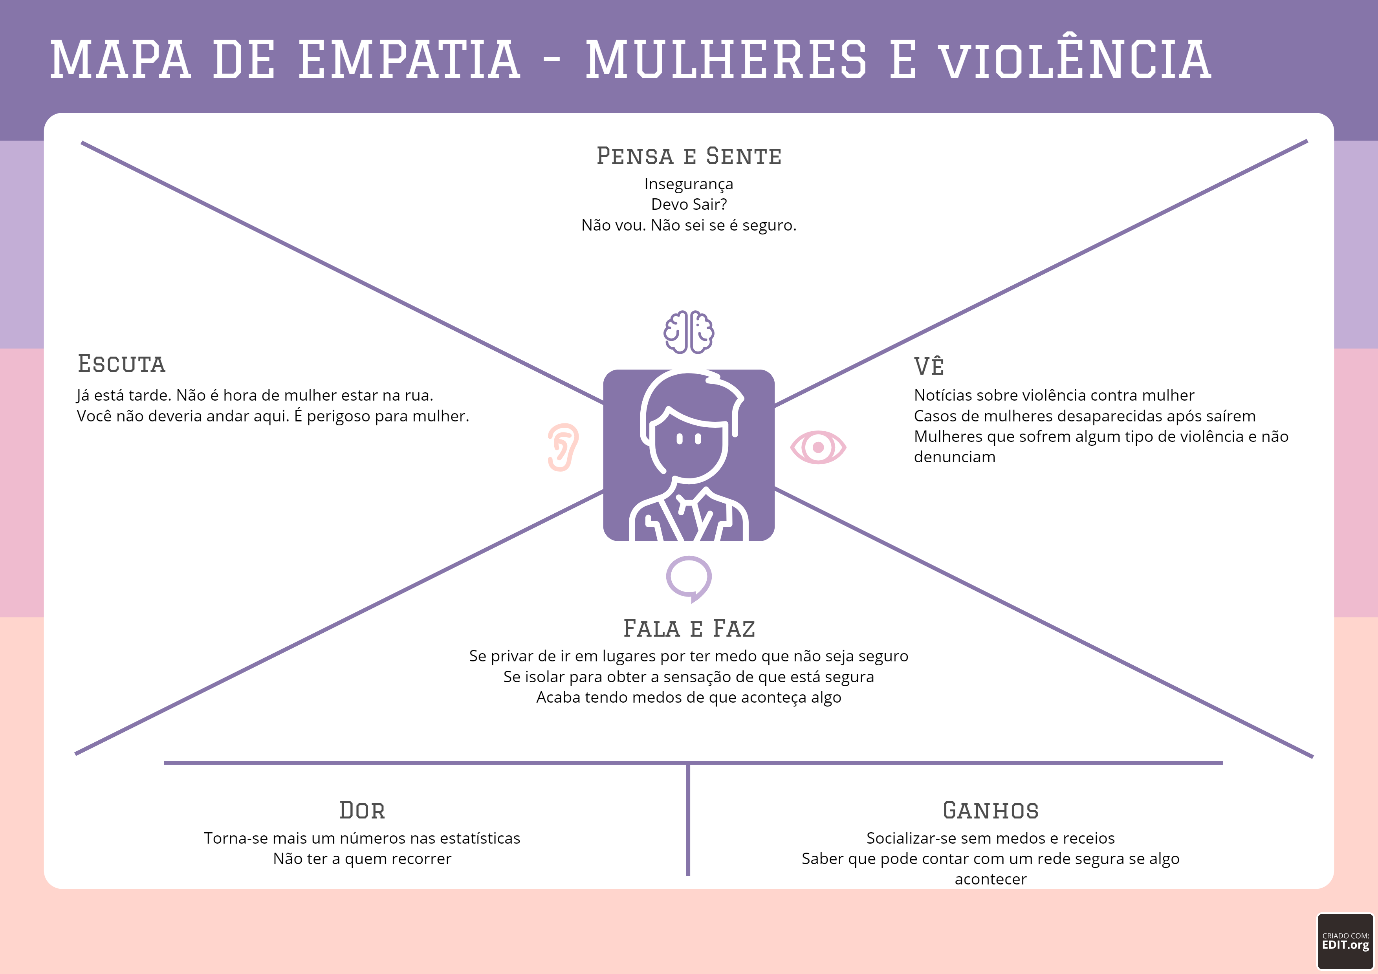
\includegraphics[width=.9\linewidth]{images/mapa-empatia-inicial.png}\\
  \end{center}
  \caption[Mapa de empatia inicial]{Mapa de empatia inicial sobre sentimento das mulheres sobre violência}
  \label{fig:mapa-empatia=inicial}
  \legend{Fonte: Próprio Autor}
\end{figure}

\section{Ambiente de uso}
O SheSafe poderá ser utilizado em qualquer ambiente desde que se tenha um plano de internet ativo para que os pedidos de ajuda possam ser enviados corretamente para a lista de contatos seguros. Uma outra restrição quanto ao uso é que os usuários devem possuir um smartphone com sistema operacional Android ou iOS para que possam instalar o aplicativo.

\section{Restrições de Uso/Circunstâncias}
Não há restrições quanto ao uso do SheSafe. Caso o usuário sinta-se em situação de risco ele poderá acionar o aplicativo e enviar seu pedido de ajuda, desde que já tenha cadastrado sua lista de contatos seguros.

\section{Diferencial}
Dado que muito dos casos de agressão acontecem com mulheres em situação de risco e muitas das vezes elas são privadas de acesso a formas de comunicação mais tecnológicas, o intuito é ter uma aplicação onde as mulheres possam reportar crimes de forma simples, prática e disponível para todos os públicos. O principal diferencial está em não restringir o acesso a aplicação para nosso público-alvo e ter a opção de envio da localização no momento do acontecimento.

\section{Funcionalidades mínimas para garantir a relevância do aplicativo}
As funcionalidades mínimas elencadas para que o projeto tenha relevância são:
\begin{alineas}
  \item Login: Para criação de usuário
  \item Pedido de socorro: Botão para acionar pedido de socorro
  \item Lista Segura: Gerenciamento de contatos seguros
  \item Perfil: Página para alteração da mensagem de socorro

\end{alineas}

\chapter{Referencial Teórico}\label{sec:RefTeorico}
\section{Sistema operacional Android}

O Android constitui-se como um sistema operacional fundamentado no núcleo Linux, atualmente sob desenvolvimento e manutenção da empresa Google Inc. \cite{google2023}. Este sistema operacional caracteriza-se por uma arquitetura de interface baseada em manipulação direta, sendo especificamente projetado para atender às demandas de dispositivos móveis equipados com tecnologia de tela sensível ao toque, incluindo smartphones e tablets \cite{burnette2021}.

A versatilidade da plataforma Android estende-se para além dos dispositivos móveis convencionais, abrangendo uma ampla gama de equipamentos tecnológicos. Neste contexto, destacam-se as adaptações específicas como o Android TV para televisores inteligentes, o Android Auto para sistemas automotivos e o Android Wear para dispositivos vestíveis, particularmente relógios inteligentes \cite{ableson2022}. O sistema utiliza recursos de interface intuitiva, empregando a tecnologia de tela sensível ao toque para permitir que os usuários manipulem objetos virtuais através de gestos diretos, complementada por um teclado virtual integrado.

Embora o Android tenha sido concebido primordialmente para dispositivos com interface touchscreen, sua aplicabilidade transcende esta categoria, sendo implementado em consoles de videogames, câmeras digitais, computadores pessoais e diversos outros equipamentos eletrônicos \cite{murphy2023}. Esta flexibilidade arquitetural demonstra a robustez e adaptabilidade da plataforma para diferentes contextos de uso.

\subsection{Posicionamento no Mercado Global}

Dados estatísticos revelam a significativa penetração do sistema Android no mercado mundial de sistemas operacionais. Segundo levantamento conduzido pela StatCounter Global Stats \cite{statcounter2017}, empresa especializada em pesquisas e análises estatísticas de mercado tecnológico, em março de 2017, os usuários do Android representavam 37,93\% da atividade global em redes, superando ligeiramente o sistema Windows, que registrou 37,91\% no mesmo período. Estes números consolidaram o Android como o sistema operacional mais utilizado mundialmente, marcando um ponto de inflexão significativo no panorama tecnológico global.

No âmbito do desenvolvimento de aplicações móveis, pesquisa conduzida entre programadores durante o período de abril a maio de 2013 evidenciou que 71\% dos desenvolvedores direcionavam seus esforços para a plataforma Android \cite{developereconomics2013}. Esta preferência dos desenvolvedores reflete tanto a popularidade do sistema quanto as oportunidades de mercado que a plataforma oferece.

\subsection{Características de Licenciamento e Código Aberto}

Um aspecto fundamental que distingue o Android de outros sistemas operacionais móveis refere-se ao seu modelo de licenciamento. O sistema operacional distribuído pela Google opera sob licença de código aberto (open source), fundamentada na Apache License 2.0 \cite{opensource2023}, garantindo aos desenvolvedores e programadores os direitos fundamentais de estudar, modificar e distribuir o software de forma gratuita.

Esta característica de código aberto proporciona liberdade significativa para qualquer indivíduo ou organização utilizar o sistema para qualquer finalidade, sem restrições de uso comercial ou não comercial. No entanto, é importante destacar que, embora o núcleo do sistema Android seja distribuído como software livre, a maioria dos dispositivos comerciais são lançados com uma combinação híbrida de software livre e software proprietário, incluindo aplicativos e serviços específicos do fabricante ou do Google \cite{lee2022}.

\section{Android Studio}
\subsection{Caracterização e Fundamentação Técnica}

O Android Studio constitui-se como o ambiente de desenvolvimento integrado (IDE - Integrated Development Environment) oficial designado pela Google para o desenvolvimento de aplicações móveis destinadas à plataforma Android \cite{google2023androidstudio}. Esta ferramenta de desenvolvimento fundamenta-se na arquitetura do IntelliJ IDEA, uma das principais plataformas de desenvolvimento Java desenvolvida pela JetBrains, incorporando suas funcionalidades centrais de edição de código e ferramentas avançadas de desenvolvimento \cite{jetbrains2023intellij}.

A escolha do IntelliJ IDEA como base arquitetural para o Android Studio justifica-se pela robustez e maturidade desta plataforma no ecossistema de desenvolvimento Java, linguagem predominante no desenvolvimento Android tradicional. Esta decisão estratégica permitiu à Google herdar um conjunto consolidado de funcionalidades de desenvolvimento, enquanto adiciona camadas especializadas voltadas especificamente para as particularidades do desenvolvimento móvel Android \cite{meier2023android}.

\subsection{Funcionalidades e Recursos Especializados}

O Android Studio incorpora um conjunto abrangente de funcionalidades específicas para otimizar o processo de desenvolvimento de aplicações Android, transcendendo as capacidades básicas de edição de código. Entre os recursos mais significativos para a produtividade do desenvolvedor, destacam-se elementos fundamentais que caracterizam a modernidade e eficiência da plataforma.

O sistema de compilação integrado baseia-se na ferramenta Gradle, um sistema de automação de build de código aberto que oferece flexibilidade superior aos sistemas tradicionais baseados em XML, como o Apache Maven \cite{gradle2023build}. Esta integração proporciona gerenciamento automatizado de dependências, compilação incremental e configuração modular de projetos, elementos essenciais para o desenvolvimento escalável de aplicações complexas.

A plataforma incorpora um emulador Android de alta performance, desenvolvido com tecnologias de virtualização otimizadas que permitem a simulação eficiente de diversos dispositivos Android sem a necessidade de hardware físico \cite{google2023emulator}. Este recurso é fundamental para testes de compatibilidade e validação de funcionalidades em diferentes configurações de hardware e versões do sistema operacional.

O ambiente oferece suporte unificado para desenvolvimento direcionado a múltiplas categorias de dispositivos Android, incluindo smartphones, tablets, dispositivos vestíveis (wearables), sistemas automotivos e televisores inteligentes. Esta abordagem unificada simplifica significativamente o processo de desenvolvimento para ecossistemas heterogêneos de dispositivos \cite{ableson2023multiplatform}.

\subsection{Recursos de Desenvolvimento Ágil e Qualidade de Código}

O Android Studio implementa funcionalidades avançadas voltadas para metodologias de desenvolvimento ágil e manutenção da qualidade de código. O recurso Instant Run representa uma inovação significativa no ciclo de desenvolvimento, permitindo a aplicação de alterações de código diretamente em aplicações em execução, eliminando a necessidade de recompilação completa do arquivo APK (Android Package) \cite{google2022instantrun}. Esta funcionalidade reduz substancialmente o tempo de iteração durante o processo de desenvolvimento e depuração.

A integração nativa com sistemas de controle de versão, particularmente o GitHub, facilita a colaboração em equipes de desenvolvimento e o gerenciamento de código fonte \cite{github2023integration}. Adicionalmente, a plataforma disponibiliza modelos de código pré-configurados (code templates) que aceleram o desenvolvimento de funcionalidades comuns e promovem a padronização de práticas de codificação.

O ambiente incorpora um conjunto robusto de ferramentas e frameworks para implementação de testes automatizados, abrangendo testes unitários, testes de integração e testes de interface do usuário \cite{junit2023android}. Estas funcionalidades são complementadas por ferramentas especializadas de análise estática de código, capazes de identificar potenciais problemas relacionados a performance, usabilidade, compatibilidade entre versões do Android e outras questões críticas para a qualidade da aplicação final \cite{android2023lint}.

\iffalse
\begin{figure}[htbp]
  \begin{center}
  
\includegraphics[width=.5\linewidth]{images/logo-ifsp.png}\\
  \end{center}
  \caption[Exemplo de Figura]{Exemplo de inserção de figura no \LaTeX. A legenda deve vir abaixo da figura. Pode usar o comando \texttt{\textbackslash legend} ou \texttt{\textbackslash fonte} para inserir a fonte da figura. Observe que na lista de ilustrações foi utilizado o nome curto fornecido como parâmetro do caption da figura (veja o arquivo fonte .tex) ao invés dessa legenda estupidamente extensa feita de forma proposital}
  \label{fig:logo}
  \legend{Fonte: Próprio Autor}
\end{figure}
\fi
\section{Firebase}
\subsection{Caracterização e Contextualização Histórica}

O Firebase constitui-se como uma plataforma abrangente de desenvolvimento para aplicações móveis e web, tendo sido incorporada ao portfólio de soluções da Google Inc. em outubro de 2014 através de processo de aquisição estratégica \cite{google2014firebase}. Originalmente fundada em 2011 por James Tamplin e Andrew Lee, a plataforma Firebase foi concebida com o propósito de fornecer uma infraestrutura de backend-as-a-service (BaaS) completa e de alta usabilidade, direcionada especificamente para simplificar o processo de desenvolvimento e implementação de aplicações digitais \cite{tamplin2021firebase}.

A filosofia de desenvolvimento da plataforma fundamenta-se na disponibilização de um ecossistema integrado de serviços diversos, que abrangem desde funcionalidades básicas de armazenamento de dados até recursos avançados de análise comportamental e engajamento de usuários \cite{firebase2023docs}. Esta abordagem holística visa reduzir a complexidade técnica tradicionalmente associada ao desenvolvimento de backends customizados, permitindo que desenvolvedores concentrem seus esforços na criação de interfaces e experiências de usuário diferenciadas.

\subsection{Interface de Gerenciamento e Implementação}

A operacionalização da plataforma Firebase é mediada por um console web especializado, denominado Firebase Console, que representa a interface principal de gerenciamento e configuração de projetos \cite{google2023console}. Este ambiente de desenvolvimento integrado foi projetado seguindo princípios de experiência do usuário (UX) orientados à simplicidade e intuitividade, proporcionando aos desenvolvedores um fluxo de trabalho otimizado para implementação de recursos.

O processo de utilização inicia-se com a criação de um projeto no console, seguido pela seleção e configuração dos serviços desejados a partir de um catálogo extenso de funcionalidades disponíveis. Cada serviço oferecido pela plataforma é acompanhado de documentação técnica detalhada, incluindo guias de implementação passo-a-passo, exemplos de código e melhores práticas de desenvolvimento \cite{firebase2023implementation}.

\subsection{Modelo de Comercialização e Estrutura Tarifária}

O Firebase opera sob um modelo de negócios freemium, caracterizado pela disponibilização gratuita de funcionalidades básicas combinada com planos pagos para recursos avançados e maior capacidade de processamento \cite{google2023pricing}. Esta estrutura tarifária escalonável permite que desenvolvedores individuais e pequenas equipes iniciem projetos sem investimento inicial, enquanto organizações com demandas mais robustas podem optar por planos comerciais adequados às suas necessidades específicas.

A estratégia de precificação adotada segue uma lógica de pay-as-you-scale, onde os custos são proporcionais ao volume de utilização dos recursos, incluindo métricas como número de usuários ativos, volume de dados armazenados e quantidade de operações de leitura/escrita realizadas \cite{moroney2022firebase}. Esta abordagem visa garantir a viabilidade econômica tanto para projetos em fase inicial quanto para aplicações consolidadas com grande base de usuários.

\subsection{Firebase Authentication}

\subsubsection{Caracterização do Serviço e Arquitetura Funcional}

O Firebase Authentication constitui-se como um serviço especializado de autenticação e autorização de usuários, integrado ao ecossistema da plataforma Firebase, oferecendo uma solução abrangente de gerenciamento de identidade digital para aplicações móveis e web \cite{google2023firebaseauth}. Este serviço fundamenta-se em uma arquitetura de backend-as-a-service (BaaS) que disponibiliza infraestrutura completa de autenticação, eliminando a necessidade de desenvolvimento e manutenção de sistemas proprietários de gerenciamento de credenciais por parte dos desenvolvedores.

A arquitetura do Firebase Authentication baseia-se na provisão de serviços de backend robustos, complementados por kits de desenvolvimento de software (SDKs) otimizados e bibliotecas de interface de usuário pré-desenvolvidas \cite{firebase2023sdk}. Esta abordagem integrada visa simplificar significativamente o processo de implementação de funcionalidades de autenticação, permitindo que desenvolvedores foquem na lógica de negócio específica de suas aplicações, enquanto delegam a complexidade técnica da autenticação para a infraestrutura especializada do Firebase.

\subsubsection{Modalidades de Autenticação e Provedores de Identidade}

O sistema oferece suporte abrangente a múltiplas modalidades de autenticação, atendendo às diversas preferências e contextos de uso dos usuários finais. A plataforma implementa autenticação tradicional baseada em credenciais de senha, permitindo que usuários criem contas através de endereços de email e senhas personalizadas \cite{stallings2023cryptography}. Adicionalmente, o serviço incorpora funcionalidades de autenticação por meio de números de telefone, utilizando protocolos de verificação por SMS para validação de identidade.

Uma característica distintiva do Firebase Authentication reside em sua capacidade de integração com provedores de identidade federados, implementando o conceito de Single Sign-On (SSO) através de plataformas estabelecidas no mercado \cite{jones2022federated}. Entre os provedores suportados, destacam-se o Google, Facebook, Twitter, GitHub, Apple, Microsoft, Yahoo, além de suporte para provedores customizados através de protocolos padronizados. Esta diversidade de opções de autenticação visa atender às preferências individuais dos usuários e reduzir barreiras de entrada nas aplicações.

\subsubsection{Integração Sistêmica e Conformidade com Padrões da Indústria}

O Firebase Authentication foi projetado com foco na integração estreita com outros componentes do ecossistema Firebase, incluindo Firebase Firestore, Firebase Realtime Database, Firebase Cloud Functions e Firebase Analytics \cite{firebase2023ecosystem}. Esta integração sistêmica permite a implementação de regras de segurança baseadas em identidade de usuário, controle de acesso granular a recursos e personalização de experiências com base no perfil de autenticação.

A arquitetura do serviço fundamenta-se na aderência rigorosa a padrões industriais reconhecidos para autenticação e autorização, particularmente os protocolos OAuth 2.0 e OpenID Connect \cite{hardt2012oauth}. O OAuth 2.0 constitui-se como o padrão de facto para autorização de aplicações web e móveis, proporcionando mecanismos seguros para concessão de acesso limitado a recursos sem exposição de credenciais. Complementarmente, o OpenID Connect representa uma camada de identidade construída sobre o OAuth 2.0, fornecendo informações de identidade de usuário de forma padronizada \cite{sakimura2014openid}.

Esta conformidade com padrões estabelecidos facilita significativamente a integração do Firebase Authentication com sistemas de backend existentes, APIs de terceiros e infraestruturas corporativas, garantindo interoperabilidade e reduzindo a complexidade de implementação em arquiteturas híbridas ou migrações graduais de sistemas legados.


\subsection{Firebase Firestore}
\subsubsection{Caracterização e Arquitetura do Sistema}

O Firebase Firestore constitui-se como um banco de dados NoSQL (Not Only SQL) orientado a documentos, desenvolvido e mantido pela Google como componente central do ecossistema Firebase \cite{google2023firestore}. Esta solução de armazenamento fundamenta-se em uma arquitetura distribuída e escalável, projetada especificamente para atender às demandas de aplicações móveis e web modernas que requerem sincronização de dados em tempo real entre múltiplos clientes e dispositivos \cite{chang2008bigtable}.

A arquitetura do Firestore baseia-se no modelo de dados orientado a documentos, onde as informações são organizadas em estruturas hierárquicas compostas por coleções e documentos \cite{mongodb2023nosql}. Cada documento representa uma unidade de dados estruturada em formato JSON, contendo pares chave-valor que podem incluir tipos primitivos, arrays, objetos aninhados e referências a outros documentos. Esta flexibilidade estrutural permite a modelagem eficiente de dados complexos sem as restrições impostas pelos esquemas rígidos dos bancos de dados relacionais tradicionais.

\subsubsection{Funcionalidades de Sincronização e Tempo Real}

Uma característica distintiva do Firestore reside em suas capacidades de sincronização automática e atualizações em tempo real \cite{firebase2023realtime}. O sistema implementa listeners de dados que permitem às aplicações cliente receber notificações instantâneas sempre que ocorrem alterações nos dados armazenados, eliminando a necessidade de polling manual ou requisições periódicas para verificação de atualizações. Esta funcionalidade é fundamental para o desenvolvimento de aplicações colaborativas, sistemas de mensagens instantâneas e interfaces que requerem refletir mudanças de estado imediatas.

O mecanismo de sincronização offline representa outro aspecto tecnológico significativo, permitindo que aplicações continuem operando mesmo durante períodos de conectividade intermitente ou ausente \cite{terry2013replicated}. O Firestore mantém uma cache local dos dados utilizados pela aplicação, sincronizando automaticamente as alterações quando a conectividade é restabelecida, garantindo consistência eventual dos dados distribuídos.

\subsubsection{Escalabilidade e Modelo de Precificação}

O Firestore foi arquitetado para proporcionar escalabilidade horizontal automática, adaptando-se dinamicamente ao volume de dados e quantidade de operações sem intervenção manual dos desenvolvedores \cite{google2023scalability}. Esta característica é particularmente relevante para aplicações com padrões de uso imprevisíveis ou crescimento exponencial de usuários, onde a capacidade de processamento deve ajustar-se automaticamente à demanda.

O modelo de precificação adotado segue uma estrutura pay-per-operation, onde os custos são calculados com base no número de operações de leitura, escrita e exclusão realizadas, complementado por tarifas de armazenamento e transferência de dados \cite{firebase2023pricing}. Esta abordagem granular de cobrança permite otimização de custos através do design eficiente de consultas e estratégias de cache, tornando-se economicamente viável tanto para projetos em escala reduzida quanto para aplicações empresariais de grande porte.

\chapter{Trabalhos Relacionados}\label{sec:TrabRel}

\chapter{Medodologia e Cronograma}\label{sec:metodos}

O abn\TeX\ introduziu o comando \texttt{IBGEtab} para formatação de tabelas. Um exemplo de tabela convencional do \LaTeX\ pode ser observado na \autoref{tab:cronograma} enquanto um exemplo usando o \texttt{IBGEtab} é mostrado na Tabela \ref{tab:cronogramaIBGE}.

\begin{table}[htbp]
  \centering
    \caption[Cronograma Normal]{Cronograma do Projeto em Meses}
    \label{tab:cronograma}
    \begin{tabular}{lcccccccccccc} %|c|c|c|c|c|c|c|c|c|c|c|c
    \toprule
    \textbf{Atividade} & \textbf{1} & \textbf{2} & \textbf{3} & \textbf{4} & \textbf{5} & \textbf{6} & \textbf{7} & \textbf{8} & \textbf{9} & \textbf{10} & \textbf{11} & \textbf{12} \\
    \midrule
        Revisão Bibliográfica & $\bullet$ & $\bullet$ & & & & & & & & & & \\
        Métodos & & & $\bullet$ & $\bullet$ & & & & & & & & \\
        Testes & & & & $\bullet$ & $\bullet$ & $\bullet$ & & & & & & \\
        Resultados & & & & & & & $\bullet$ & $\bullet$ & & & & \\
        Conclusão & & & & & & & $\bullet$ & $\bullet$ & $\bullet$ & & & \\
        Banca & & & & & & &&&& $\bullet$ & $\bullet$ & $\bullet$ \\
    \bottomrule
    \end{tabular}%
    \fonte{Próprio Autor}
\end{table}%



\begin{table}[htbp]
    \IBGEtab{
    \caption[Cronograma (IBGE)]{Cronograma do Projeto em Meses usando o comando IBGEtab para a formatação da tabela}
    \label{tab:cronogramaIBGE}
    }{
    \begin{tabular}{lcccccccccccc} %|c|c|c|c|c|c|c|c|c|c|c|c
    \toprule
    \textbf{Atividade} & \textbf{1} & \textbf{2} & \textbf{3} & \textbf{4} & \textbf{5} & \textbf{6} & \textbf{7} & \textbf{8} & \textbf{9} & \textbf{10} & \textbf{11} & \textbf{12} \\
    \midrule
        Revisão Bibliográfica & $\bullet$ & $\bullet$ & & & & & & & & & & \\
        Métodos & & & $\bullet$ & $\bullet$ & & & & & & & & \\
        Testes & & & & $\bullet$ & $\bullet$ & $\bullet$ & & & & & & \\
        Resultados & & & & & & & $\bullet$ & $\bullet$ & & & & \\
        Conclusão & & & & & & & $\bullet$ & $\bullet$ & $\bullet$ & & & \\
        Banca & & & & & & &&&& $\bullet$ & $\bullet$ & $\bullet$ \\
    \bottomrule
    \end{tabular}%
    }{
    \fonte{Próprio Autor}}
\end{table}%


\chapter{Resultados Esperados}\label{sec:resultEsperados}


% ----------------------------------------------------------
% ELEMENTOS PÓS-TEXTUAIS
% ----------------------------------------------------------
\postextual

% Referências bibliográficas

\bibliography{referencias}

% Caso sejam necessários apêndices ou anexos em seu documento
% Use os ambientes abaixo

%% Apêndices
%
%% Inicia os apêndices
%\begin{apendicesenv}
%
%% Imprime uma página indicando o início dos apêndices
%\partapendices
%
%\chapter{Primeiro Apêndice}
%
%\chapter{Segundo Apêndice}
%
%\end{apendicesenv}
%
%
%% ----------------------------------------------------------
%% Anexos
%% ----------------------------------------------------------
%\begin{anexosenv}
%
%% Imprime uma página indicando o início dos anexos
%\partanexos
%
%\chapter{Primeiro Anexo}
%\lipsum[30]
%
%\chapter{Segundo Anexo}
%\lipsum[31]
%
%\end{anexosenv}

\end{document}
